\chapter{Especificación de la arquitectura}

\section{Arquitectura del sistema}

\begin{figure}[!htb]
	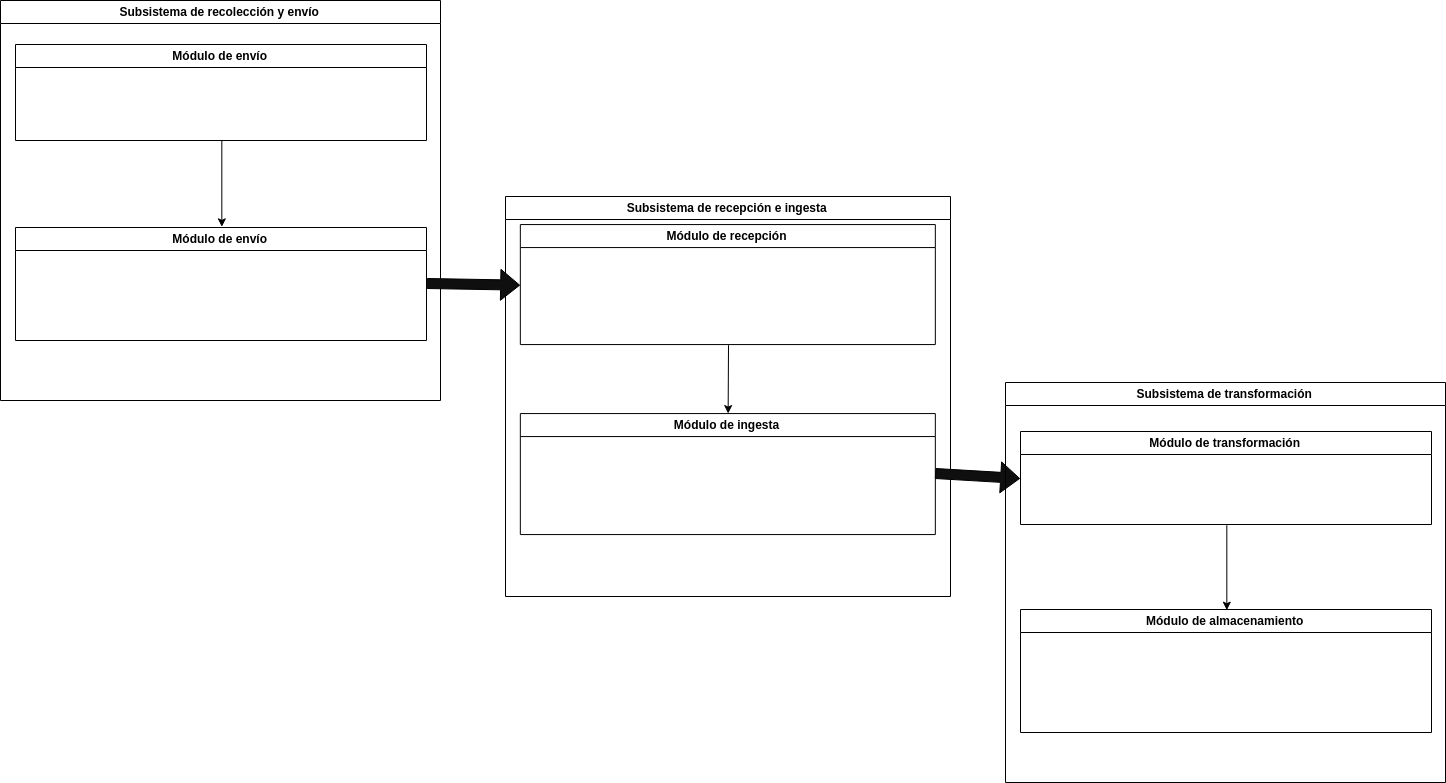
\includegraphics[width=\linewidth] {Moduloss-arquitecturaparcial.png}
	\caption{Vista parcial de la arquitectura del sistema}
	\label{fig:arqparcial}
\end{figure}

La arquitectura del sistema se divide en tres partes o subsistemas, cada subsistema tiene una tarea diferenciada dentro del sistema. En la figura \ref{fig:arqparcial} se puede ver una vista parcial de como se relacionan los subsistemas y los módulos del sistema. Las flechas indican el sentido del flujo de datos.
 
 
 Los subsistemas son los siguientes:

\begin{itemize}
	\item \textit{Subsistema de recolección y envío}: Está compuesto de dos módulos, el de recolección y el de envío. El módulo de recolección se encarga de recoger los eventos en el dispositivo ubicuo. El módulo de envío se encarga de enviar los eventos recogidos por el módulo de recolección al módulo de recepción del subsistema de recepción e ingesta.
	
	\item \textit{Subsistema de recepción e ingesta}: Está compuesto por dos módulos, el de recepción y el de ingesta. El módulo de recepción se encarga de centralizar la ingesta de eventos a un único punto de entrada y  de recibir los eventos que le envía el módulo de envío. El módulo de ingesta se encarga de recibir los eventos del módulo de recepción y almacenarlos como mínimo hasta que el módulo de transformación los consuma.

	\item \textit{Subsistema de transformación}:  Está compuesto por dos módulos, el de transformación y el de almacenamiento. El módulo de transformación se encarga de transformar los eventos que consume del módulo de ingesta y de enviarlos al módulo de almacenamiento. El módulo de almacenamiento recibe los eventos transformados del módulo de transformación y los almacena.
\end{itemize}

La arquitectura propuesta cumple con las fases del proceso ETL. Los encargados de la Extracción son el subsistema de recolección y envío, y el subsistema de recepción e ingesta. El encargado de la Transformación y la Carga es el subsistema de transformación.

Esta arquitectura está basada en la arquitectura Kappa\cite{Tfg:kappa}, siendo el módulo de ingesta el que implemente la capa de almacenamiento de datos, el módulo de transformación el que implemente la capa de Stream Processing y el módulo de almacenamiento el que implemente la capa en la cual se sirven los datos.

